\documentclass[12pt]{article}
\usepackage{amsmath}
\usepackage{graphicx,psfrag,epsf,float, bm}
\graphicspath{C:/Users/Colin/Documents/GitHub/BB_data_analysis/paper/fig/}
\usepackage{enumerate}
\usepackage[numbers]{natbib}
\usepackage{url} % not crucial - just used below for the URL

% no longer require relative path to figs
\graphicspath{{fig/}}

\usepackage[x11names]{xcolor}
\usepackage{framed} % provides framed env., should be removed in final draft
\definecolor{shadecolor}{rgb}{1,.5,.5}

% math macros 

\newcommand{\ind}{\stackrel{ind.}{\sim}}
\newcommand{\op}{\operatorname}
\DeclareMathOperator*{\argmin}{arg\,min}
\newcommand{\myequation}{\begin{equation}}
\newcommand{\myendequation}{\end{equation}}
\let\[\myequation
\let\]\myendequation


\pdfminorversion=4
% NOTE: To produce blinded version, replace "0" with "1" below.
\newcommand{\blind}{0}

% DON'T change margins - should be 1 inch all around.
\addtolength{\oddsidemargin}{-.5in}%
\addtolength{\evensidemargin}{-.5in}%
\addtolength{\textwidth}{1in}%
\addtolength{\textheight}{1.3in}%
\addtolength{\topmargin}{-.8in}%


\begin{document}

\def\spacingset#1{\renewcommand{\baselinestretch}%
{#1}\small\normalsize} \spacingset{1}


%%%%%%%%%%%%%%%%%%%%%%%%%%%%%%%%%%%%%%%%%%%%%%%%%%%%%%%%%%%%%%%%%%%%%%%%%%%%%%

\if0\blind
{
  \title{\bf A Hierarchical Bayesian Approach for Modeling Infant-Mortality and Wearout Failure Modes}
  \author{Eric Mittman\thanks{
    The authors gratefully acknowledge Bill Meeker for his comments and suggestions}\hspace{.2cm}\\
    Department of Statistics, Iowa State University\\
    and \\
    Colin Lewis-Beck \\
    Department of Statistics, Iowa State University}
  \maketitle
} \fi

\if1\blind
{
  \bigskip
  \bigskip
  \bigskip
  \begin{center}
    {\LARGE\bf Title}
\end{center}
  \medskip
} \fi

\bigskip
\begin{abstract}
% Consumers have an interest in accurate assessment of product reliability.  However, lifetime data is often sparse and has limited information.  
When the information carried by lifetime data are limited by sample size, censoring and truncation, lifetime analysis can suffer from imprecision. These limitations are not atypical; for example, lifetime data for high-reliability products will tend to be right-censored.

With field data on consumer products, model-based appproaches to inference require a model with sufficient flexibility to account for multiple kinds of failure. The causes of these, while not interesting to the consumer per se, can lead to various observed lifetime distributions. Because of this, standard lifetime models, such as Weibull or lognormal may be inadequate. 

In this paper we present a method for joint estimation of multiple lifetime distributions based on the Generalized Limited Failure Population (GLFP) model \citep{chan}. This 5-parameter model for lifetime data accommodates lifetime distributions with multiple failure modes:  early failure due to "infant mortality" and failure due to wearout. We fit the GLFP model using a hierarchical modeling approach.  Borrowing strength across populations, our method enables estimation with uncertainty of lifetime distributions even in cases where the number of model parameters is larger than the number of observed failures.  Moreover, using our Bayesian method, comparison of different product brands is straightforward because estimation of arbitrary functionals are easily computable using samples from the posterior distribution.
\end{abstract}

\noindent%
{\it Keywords:} GLFP, Bathtub hazard, Censored data, Hierarchical models, Bayesian estimation
\vfill

\newpage
\tableofcontents
\newpage
\spacingset{1.45} % DON'T change the spacing!
\section{Introduction}
Consumers have an interest in accurate assessment of product reliability. Toward this end, there is a need for models that can accomodate common failure patterns and methods which can make the most of available data and properly account for uncertainty.
%While computationally convenient, simple lifetime models can fail at each of these.

The reliability of many engineered products follow a similar pattern. Relatively high rates of failure occurring early ("infant mortality") due to manufacturing defects.  After this "burn-in" period, failure rates stabilize as the majority of defective units have failed and are no longer in the population.  Finally, after prolonged use, rates of failure increase due to wearout.  Ignoring this pattern in failure rates can lead to suboptimal decisions and spurious inferences about a product's reliability. This highlights the importance of choosing a sufficiently flexible model.

Nonparametric methods require relatively few assumptions, but they are not suitable for forecasting. Moreover, nonparametric estimates made using small samples, or data which are heavily censored may be too noisy to be practical. Appropriate parametric models can make better use of available data. For inference, likelihood-based methods are well-equipped to deal with truncated and/or censored data. Furthermore, by assuming a parsimonious representation of the data-generating process, parametric models admit simpler, more intuitive ways to compare populations of interest, borrow strength across groups, and incorporate prior information. 

Often no information is available to identify why a unit failed. This presents a dilemma for analysts: the data may indicate multiple failure modes, contraindicating the use of a unimodal parametric distribution. However, without any knowledge of cause of failure, traditional competing risk models are not identifiable. \citet{chan} proposed the Generalized Limited Failure Population (GLFP) model. This model can provide a solution to the problem of unknown cause of failure (masking) in the special case where there is evidence of two modes of failure which impact different stages of product life. It avoids non-identifiability by introducing a parameter representing the population proportion defective. Where this parameter is zero, the GLFP model reduces to a unimodal distribution. \\

The GLFP model has a meaningful parameterization and accommodates lifetime data with infant mortality and wearout.  Unfortunately, it can require a lot of data to fit due to the model's complexity. When multiple sources of information are available, partial pooling, accomplished via hierarchical modeling, can reduce the amount of data required to produce stable parameter estimates. When multiple populations are of interest, comparisons based on separate, unrestricted GLFP model fits will be limited to those products with sufficient data. As we will show, hierarchical modeling of the GLFP parameters allows for borrowing of information across populations which imposes "soft" constraints on model parameters. This enables estimation of the lifetime distribution for all populations via shrinkage toward a "pooled" model, with the degree of shrinkage inversely related to the amount of population specific information. We demonstrate computation of various quantities of interest while comparing reliability across populations using numerical integration over the posterior distribution with samples obtained via  Markov Chain Monte Carlo. 

The structure of the paper is as follows.  Section~\ref{sec:Background} describes some of the potential applications of our method and summarizes previous related work found in the literature. Section~\ref{sec:GLFP model} introduces the GLFP model and illustrates an application in an example. Section~\ref{sec:Hierarchical GLFP model} introduces a hierarchical model for extending the GLFP model to multiple populations. In section~\ref{sec:Data analysis} we illustrate applying the hierarchical GLFP model to a real data set. Subsection~\ref{sec:Data} describes and summarizes the Backblaze Hard Drive data set.  Subsection~\ref{sec:Model Comparisons} shows the use of approximate leave-one-out cross-validation as a way to do model selection between different hierarchical model specifications. We also address computational issues and modeling decisions that lead to a final model.  In subsection~\ref{sec:Drive-model Comparisons} we present an analysis comparing drive-model lifetime distributions.  Finally, in section~\ref{sec:Conclusions}, we discuss the strengths and limitations of our method and consider extensions and alternatives.

\section{Background}
\label{sec:Background}
In engineering applications, a product can often fail from one out of a set of possible malfunctioning components.  For example, a computer system can break if the mother board, disc drive or power supply stop working.  Circuit boards (CB) can fail due to a manufacturing defect or later as a result of wearout.  The general name for such products is a series system where the lifetime of the product is the minimum failure time across different components or risks \cite{nelson}.  A common assumption in series systems is the time to failure for each risk is statistically independent.  Thus, the overall reliability of a unit is modeled using the product rule across all risks.  Parameter estimation is straightforward if the cause of failure is known for each observation.  However, in many situations the cause of failure is unknown to the analyst. This is referred to in the literature as "masking".\\

Previous papers have employed various data assumptions and methodologies to model masked lifetime failure data.  When modeling computer system failures Reiser et al. assumed each observed failure came from a known subset of failure modes, and estimation was performed using a Bayesian approach \cite{reiser}.  Chan and Meeker labeled the cause of circuit board failures as infant mortality, unknown, or wearout based on the time of observed failures.  This helped identify parameters when using maximum likelihood (ML) estimation.  Extending Chan and Meeker's analysis, Basu et.al performed a Bayesian analysis with informative priors to better identify early versus late failure modes without making any data assumptions \cite{basu}.  Berger and Sun introduced the Poly-Weibull distribution where cause of failure is the minimum of a several Weibull distributions \cite{berger}.  More recently, Ranjan et al. considered a competing risk model for infant mortality and wearout as a mixture of Weibull and exponential failure distributions \cite{ranjan}.  Treating the unknown failure modes as incomplete data, an expectation maximization (EM) algorithm providing ML estimates was used, in addition to Bayesian estimation.


\section{Generalized Limited Failure Population model}
\label{sec:GLFP model}

\subsection{Weibull parameterization}
\label{sec:Weibull parameterization}
For a random variable $Y$ following a Weibull distribution, the standard parameterization of the cumulative distribution function, in terms of scale parameter $\alpha$ and shape parameter $\beta$, is

$$ P(Y \le y) = 1 - \exp \left\{ \left( \frac{y}{\alpha} \right)^\beta \right\}. $$

An alternative parameterization, in terms of log-location parameter $\mu = \log \alpha$ and log-scale parameter $\sigma = 1/\beta$ is

\begin{equation} P(Y \le y) = 1 - \exp \left\{ -\exp \left( \frac{ \log y - \mu }{\sigma} \right) \right\}\\
= \Phi_{SEV}\left(\frac{\log y - \mu}{\sigma}\right),
\end{equation}
where $\Phi_{SEV}$ is the cdf of the standard smallest extreme value distribution (SEV). Thus, the Weibull distribution is a log-location scale family, with $\log Y$ following an SEV distribution with location parameter $\mu$ and scale parameter $\sigma$. With this in mind, the corresponding density function is
\begin{equation}
p(y) = \frac{1}{\sigma y}\exp\left\{\frac{\log y - \mu}{\sigma} - \exp \left( \frac{\log y - \mu}{\sigma} \right)\right\}\\
=\frac{1}{\sigma y} \phi_{SEV}\left(\frac{\log y - \mu}{\sigma}\right)
\end{equation}

An advantage conferred by writing the model in this way is that the log of the $p^{th}$ quantile, $t_p$, is a linear function of the parameters, which allows an analyst to apply prior information in a straightforward way.  Using the inverse cdf of the SEV distribution,
\begin{equation}
\log t_p = \mu + \sigma \Phi_{SEV}^{-1}(p),
\end{equation}
where $t_p = \argmin\{y:\Phi_{SEV}(\log y)>p\}$. Since $\Phi(0)\approx 0.632$, $\log{\eta} = \mu  =t_{.63}$, and when there is more prior knowledge about a quantile other than $t_{.63}$, as is often the case with high-reliability products,  this representation allows the analyst to put prior distributions directly on those quantities.


\subsection{GLFP model}
\label{subsec:GLFP model}
Following \cite{chan}, let $F_1,F_2$ be Weibull distributions with parameters $(\mu_1,\sigma_1)$ and $(\mu_2, \sigma_2)$ respectively.
The Generalized Limited Failure Population model (GLFP) of \citet{chan} is defined as follows: Let $Y \sim \op{GLFP}(\pi, \mu_1,\sigma_1,\mu_2,\sigma_2)$. Then
$$P(Y \le y) = F(y) = 1 - (1-\pi\, F_{1}(y))(1 - F_{2}(y)),\, t>0,\, 0 < \pi < 1.$$

The GLFP model can be understood as a marginalized mixture model with a binary latent variable, $\delta_i\ind \op{Bernoulli}(\pi)$. $\delta_i$ is an indicator for whether or not an observational unit is defective. Expressed conditional on $\delta_i$,
\begin{align*}
P(Y\le y | \delta_i=1) =& 1 -(1-F_1(y))(1-F_2(y))\\
P(Y\le y | \delta_i=0) =& F_2(y).
\end{align*}

 
The parameter $\pi_d$ represents the proportion of units susceptible to early failure, hence susceptible to both failure modes. Here the cause of failure is not assumed to be known, thus units from the same population are exchangeable.

Taking the derivative of the (marginal) cdf, the density for the GLFP is
\begin{equation}
f(y|\pi, \mu_1,\sigma_1, \mu_2, \sigma_2) = \pi f_1(y|\mu_1,\sigma_1)\left(1-F_2(y|\mu_2,\sigma_2)\right) + f_2(y|\mu_2,\sigma_2)\left(1-\pi F_2(y|\mu_2,\sigma_2\right).
\end{equation}

\subsection{Censoring and Truncation}
A common feature of lifetime data is right-censoring. Due to time or budget constraints it is rare all units are observed until failure. If a unit has not yet failed when the data is analyzed it is considered right-censored.  In other words, right-censoring puts a lower bound on the failure time.  Lifetime data for products with long expected lifetimes, such as hard drives, have a natural tendency to exhibit right-censoring.


When an observation is left-truncated, it would not have been observed if it had failed prior to a particular time, which we refer to as the left-truncation time.  Left-truncation is a common feature of observational lifetime data, where the factors leading to inclusion in the data set are uncontrolled and/or the population of interest has a history prior to any data collection. Ignoring left truncation can lead to biased estimates. However, dropping left truncated observations should be avoided because it could substantially reduce the total available information.  Therefore, we incorporate both right censoring and left truncation into the likelihood. 


\subsubsection{Likelihood}
We now give the general form for the likelihood function, taking into account left truncation and right censoring.  Let $Y_{i}$ denote the end of the observed lifetime of unit $i$, in hours.  Let $t_i^L$ be the left truncation time; that is, the first time reported for the unit.  Additionally, let $c_i$ be an indicator for censoring; $c_i=1$ if the failure time is right-censored, $c_1=0$ if the unit failed (at time $Y_i$). The likelihood for the GLFP is a function of $\bm{\theta} = (\mu_1, \sigma_1, \mu_2, \sigma_2, \pi)$.  Assuming the lifetimes of all units are independent, the likelihood for the data, $Y_1,\ldots,Y_N$ is given by
\begin{equation*}
L(\bm{\theta})= \prod_{i=1}^{n} \left[\frac{f(y_i;\bm{\theta})}{1-F(t_i^L;\bm{\theta})}\right]^{1-c_i} \left[ \frac{1-F(y_i;\bm{\theta})}{1-F(t_i^L;\bm{\theta})} \right]^{c_i}
\end{equation*}

\subsection{Example 1}
\label{subsec:ex1}
We fit the GLFP model on real hard drive failure data from a cloud-based storage company.  Computer hard drives are known to have a mixture of early and late failures, making the GLFP an appropriate parametric model \cite{chan}.  The data contains the number of hours the hard drive was in operation, and whether the drive failed or was right censored.  No information is available about the cause of failure.  We first focus on the drive brand model with the most observed failures to demonstrate the GLFP model.  We fit the GLFP using a Bayesian framework and specified the following proper priors to ensure a proper posterior distribution.
$$t_{0.5,1} \sim \op{N}(8,4), \quad t_{0.2,2} \sim \op{N}(10,4)$$
$$\mbox{logit}^{-1}\pi_1 \sim \op{Normal}(-3,2),\quad \sigma_1 \sim \op{Lognormal}(0, 2.5), \quad \sigma_2 \sim \op{Lognormal}(0, 2.5) $$

%\begin{figure}[H]
%\centering
%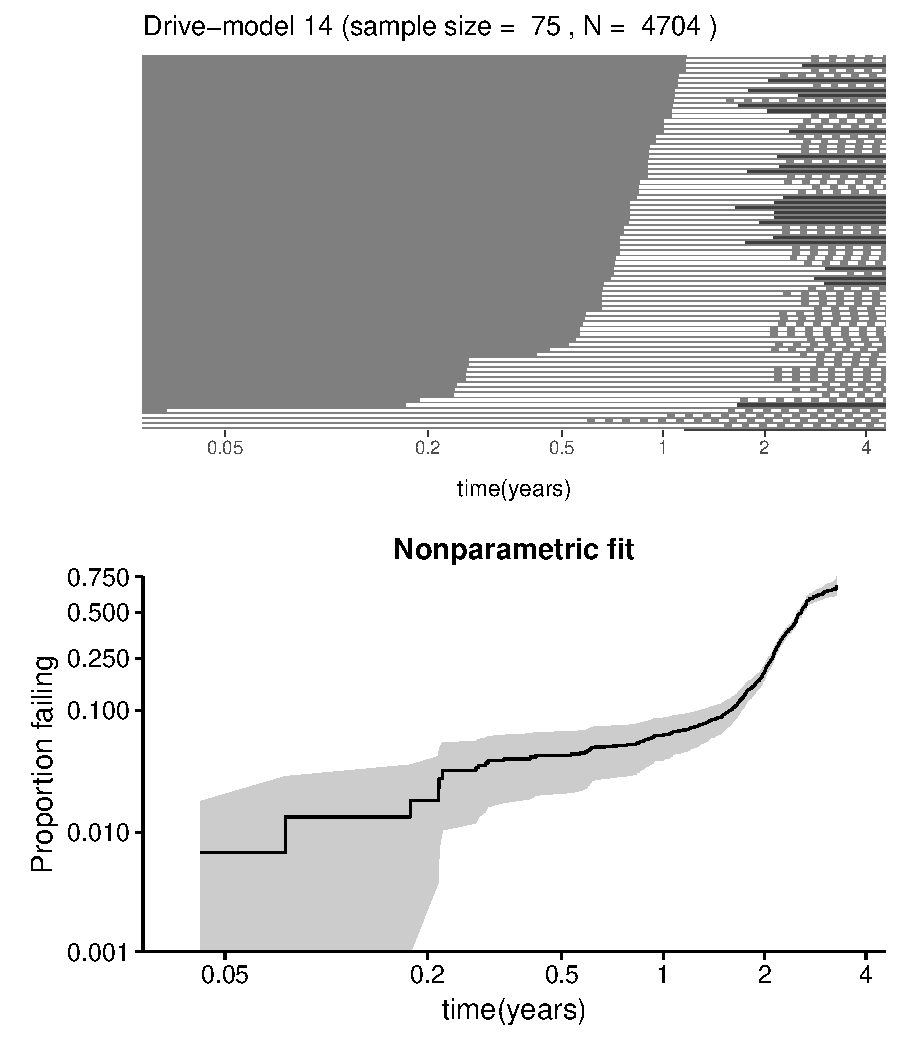
\includegraphics{np_ex1}
%\caption{Top: Lifetime plot of data from 75 randomly selected units of drive-model `14'. Bottom: Kaplan-Meier estimate for drive-model `14'.}
%\label{dm14}
%\end{figure}


The prior on $\pi$ implies with $90\%$ probability $\pi$ is in the interval $(.002, .572)$.  Given the interpretation of $\pi$ as the proportion of defective units, which we would expect to be small, a range primarily covering the left side of 0.50 is reasonable and weakly informative.  The prior on $\sigma_1$ and $\sigma_2$ put the majority of mass on the interval $(0.02, 61.1)$ with $90\%$ probability.  Again, this allows for a wide range of hazards, larger than we would expect to see in the data.  The $t_{0.5,1}$ distribution has a prior $90\%$ interval of $(1.4,14.6)$. For $t_{0.2,2}$ the range is $(3.4,16.6)$. Since these last two parameters are on the scale of log-hours, admitting values from hours to decades, we consider them to be relatively uninformative.  They do, however, help separate the early and late failure modes--the earlier infant mortality mode having a lower mean time to failure than the wearout mode.  This is helpful for estimation since, as discussed in Chan \& Meeker, ML had difficulty identifying the two sets of GLFP parameters without making strong assumptions about the data.  \\


Table 1 gives the posterior median and 95\% credible intervals for the 5 GLFP parameters for drive model 14.  The parameter $p$ is an estimate of the proportion of drives susceptible to to infant mortality.  As expected, this fraction is small with a median value of 0.05.  The parameter estimates for the two Weibull distributions also match intuition.  The wearout failure mode puts posterior probability on a values of $\beta_1$ less than 1, which corresponds to a decreasing hazard.  Conversely, the credible interval for $\beta_2$, the wearout mode, is strictly above 1, an increasing hazard.  The two means times to failure (on the log scale) are also well identified with the infant mortality failure mode having an earlier mean time to failure than the wearout mode. 

\begin{table}[H]
\centering
\begin{tabular}{rrrr}
  \hline
 & 2.5\% & 50\% & 97.5\% \\ 
  \hline
$\pi$ & 0.03 & 0.05 & 0.10 \\ 
 $\beta_1$ & 0.47 & 1.13 & 1.72 \\ 
  $\beta_2$ & 4.47 & 4.70 & 4.95 \\ 
  $\mu_1$ & 7.46 & 8.06 & 8.76 \\ 
  $\mu_2$ & 10.12 & 10.13 & 10.14 \\ 
   \hline
\end{tabular}
\caption{Posterior 95\% Credible Intervals for the 5 GLFP parameters for Drive Model 14.}
\label{table:1}
\end{table}

Probability plotting is a simple method to assess the adequacy of (log)location-scale families of probability models to the data.  After properly transforming the axes of a plot, graphing an empirical estimate of fraction failing as a function of time along with simultaneous confidence bands provides a visual check for distributional goodness of fit.  We applied this method using the Kaplan-Meier non-parametric estimate of the empirical cdf \cite{kaplan}.  With left truncation, however, the standard Kaplan-Meier estimator is biased, so we used an adjusted version (see Appendix for a more detailed description).   

In Figure 1 we plot the Kaplan-Meier adjusted cdf for drive model 14 on Weibull paper.  The solid stepwise curve corresponds to the observed failures.  Censored drives are not plotted.  Standard error bands are calculated using Greenwood's method \cite{green}.  Also plotted is the median of the posterior draws for the GLFP model along with 90\% pointwise credible interval bands.  The non-parametric and parametric model align up quite closely.  Moreover, evidence of at least two failure modes is seen in the acceleration of the hazard rate between 8000 and 20,000 hours.  Therefore, a single Weibull model is clearly not flexible enough to characterize this lifetime distribution. The discrepancy in the right tail of the distribution appears to be real. We don't provide a solution to this problem here. Certainly, if there are clearly more that two well-separated failure modes, the GLFP will not fit the data well. However, we consider it satisfactory if we can provide a good approximation to the observed lifetime distribution over the bulk of the product life. In practical terms, the right tail is of less importance for electronic goods, due to obsolescence.

\begin{figure}[H]
\centering
  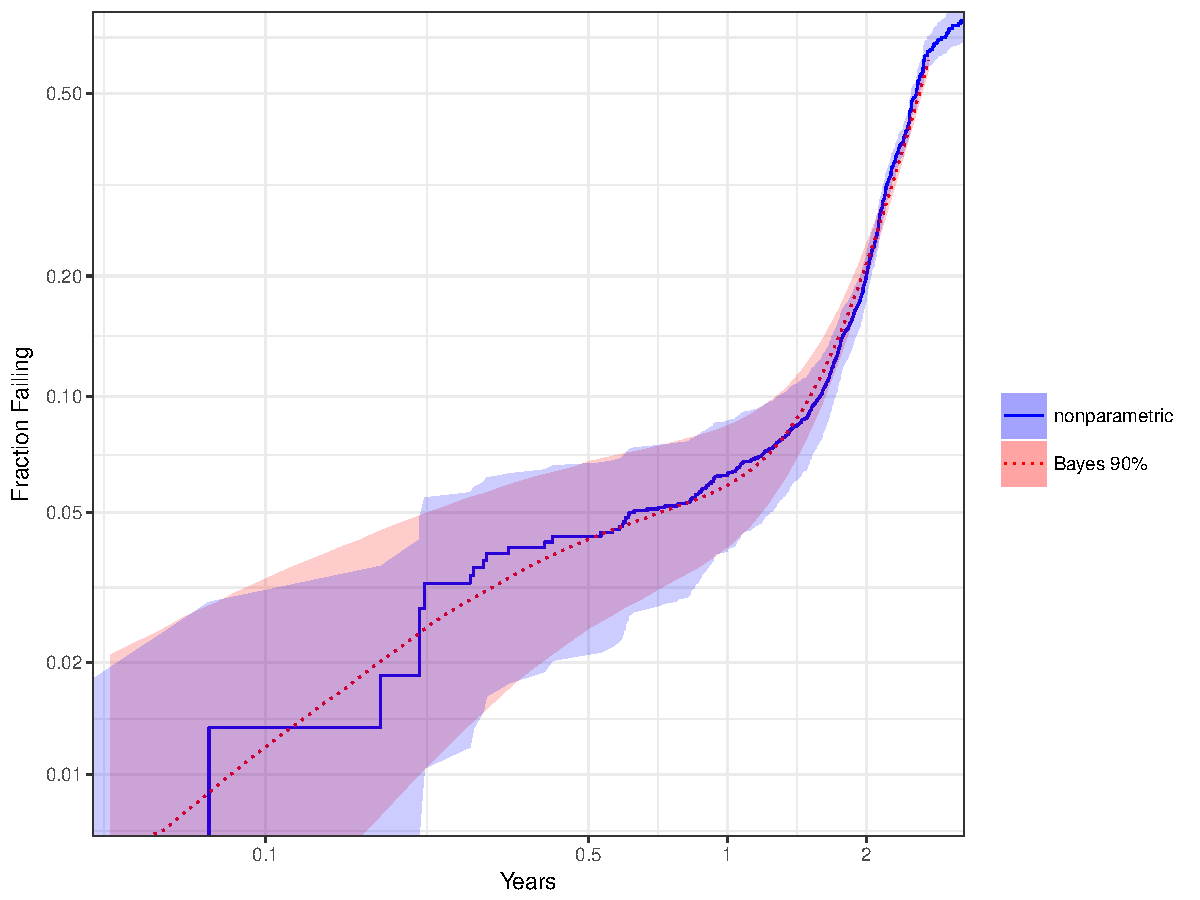
\includegraphics[width=.8\textwidth]{drive14cred.pdf}
  \caption{Estimated GLFP for drive-model 14 plotted on Weibull paper.  Dashed line corresponds to the median of the posterior draws.  Solid blue line is a non-parametric Kaplan-Meier estimator.  Credible 90\% bands are in red.  Greenwood non-parametric error bands are in blue.}
  \label{fig1}
\end{figure}


\section{Hierarchical GLFP model}
\label{sec:Hierarchical GLFP model}

To borrow strength across different populations, we can model the population specific parameters hierarchically, allowing the data to inform the hyperparameters.
%For the second option, we model the scales, $\sigma_j$, quantiles, $t_{p_j,d,j}$, and proportions, $\pi_d$, of the component distributions as follows:

Let
\begin{equation}
y_{g,i} \ind \op{GLFP}\left( \pi_g, \mu_{1g}, \sigma_{1g}, \mu_{2g}, \sigma_{2g} \right),
\end{equation}
where $g=1,\ldots,G$ indexes populations. Next we model these parameters themselves as random variables. Let
\begin{equation*}
\sigma_{1g} \ind \op{LN} \left( \eta_{\sigma_1}, \tau^2_{\sigma_1} \right)
\end{equation*}
\begin{equation*}
\sigma_{2g} \ind \op{LN} \left( \eta_{\sigma_2}, \tau^2_{\sigma_2}\right)\op{T}\left(0, 1\right)
\end{equation*}
\begin{equation}
\label{eq:hier-model}
\log t_{p_{1}g} \equiv \mu_{1g} + \sigma_{1g}\,\Phi^{-1}(p_1)  \ind \op{N} \left(\eta_{t_{p_1}}, \tau^2_{t_{p_1}}\right)
\end{equation}
\begin{equation*}
\log t_{p_{2}g} \equiv \mu_{2g} + \sigma_{2g}\,\Phi^{-1}(p_2)  \ind \op{N} \left(\eta_{t_{p_2}}, \tau^2_{t_{p_2}}\right)
\end{equation*}
\begin{equation*}
\op{logit} \pi_g \ind \op{N}(\eta_\pi, \tau_\pi).
\end{equation*}

As discussed in section \ref{sec:Weibull parameterization}, we reparameterize the Weibull in terms of log quantile and scale since the data we encounter are more informative about the left side of their respective lifetime distribution. We truncate the distribution of $\sigma_{2g}$ at $1$, restricting the wearout failure mode to have an increasing hazard function. We choose to model these parameters (or suitable transformations) with normal distributions because many populations require strong regularization which the normal, with its exponentially decreasing tails, provides. 

In principle, we prefer this full model because we tend to believe that every population has a distribution with a distinct set of parameters. In practice, however, we may consider restrictions to reduce the number of parameters if the data do not support their inclusion. For example, we may consider a model with a common $\sigma_{1}$, letting $\sigma_{1g}=\sigma_1$ for all $g=1,\ldots,G$. A practical strategy is to begin with a simple model and gradually add complexity, reevaluating model adequacy at each iteration. In section \ref{sec:Model Comparisons}, we illustrate this process, fitting a series of models with increasing complexity and evaluating their performance using a measure of leave-one-out predictive error.


\section{Real data analysis}
\label{sec:Data analysis}
\subsection{Backblaze hard drive data}
\label{sec:Data}
Backblaze is a company that offers cloud backup storage to protect against data loss.  Since 2013 it has been collecting data on hard drives operating at its facility.  The purpose is to provide consumers and businesses with reliability information on different hard drive-models.  The hard drives continuously spin in controlled storage pods.  Drives are run until failure.  When a hard drive fails it is permanently removed and replaced.  In addition, the number of storage pods is increasing as Backblaze adds to its storage capacity.  Every quarter Backblaze makes its data publicly available through their website \cite{backblaze}. In addition, Backblaze publishes summary statistics of the different hard drive-models currently operating.  No other analysis or modeling of the failure data is provided.  Backblaze does, however, encourage others to further analyze its data. 

As of the first quarter of 2016, Backblaze was collecting and reporting data on 63 different drive-models.  Some drive-models have been running since 2013 or before, while others were added at a later date.  Data have been reported on 75,297 different hard drives that are or where in operation.  The distribution of drives by drive-model varies: some drive-models have only have a service record for a single drive whereas the maximum number of daily service records for a single drive model is 35,860.  Figure \ref{fig1} shows a scatterplot of the total observed running time in hours versus the total number of failures for drive-models with at least 3 failures.  For model identification, a minimum of three failures was the criterion for hard drive brands to be included in our analyses.  

\begin{figure}[H]
  %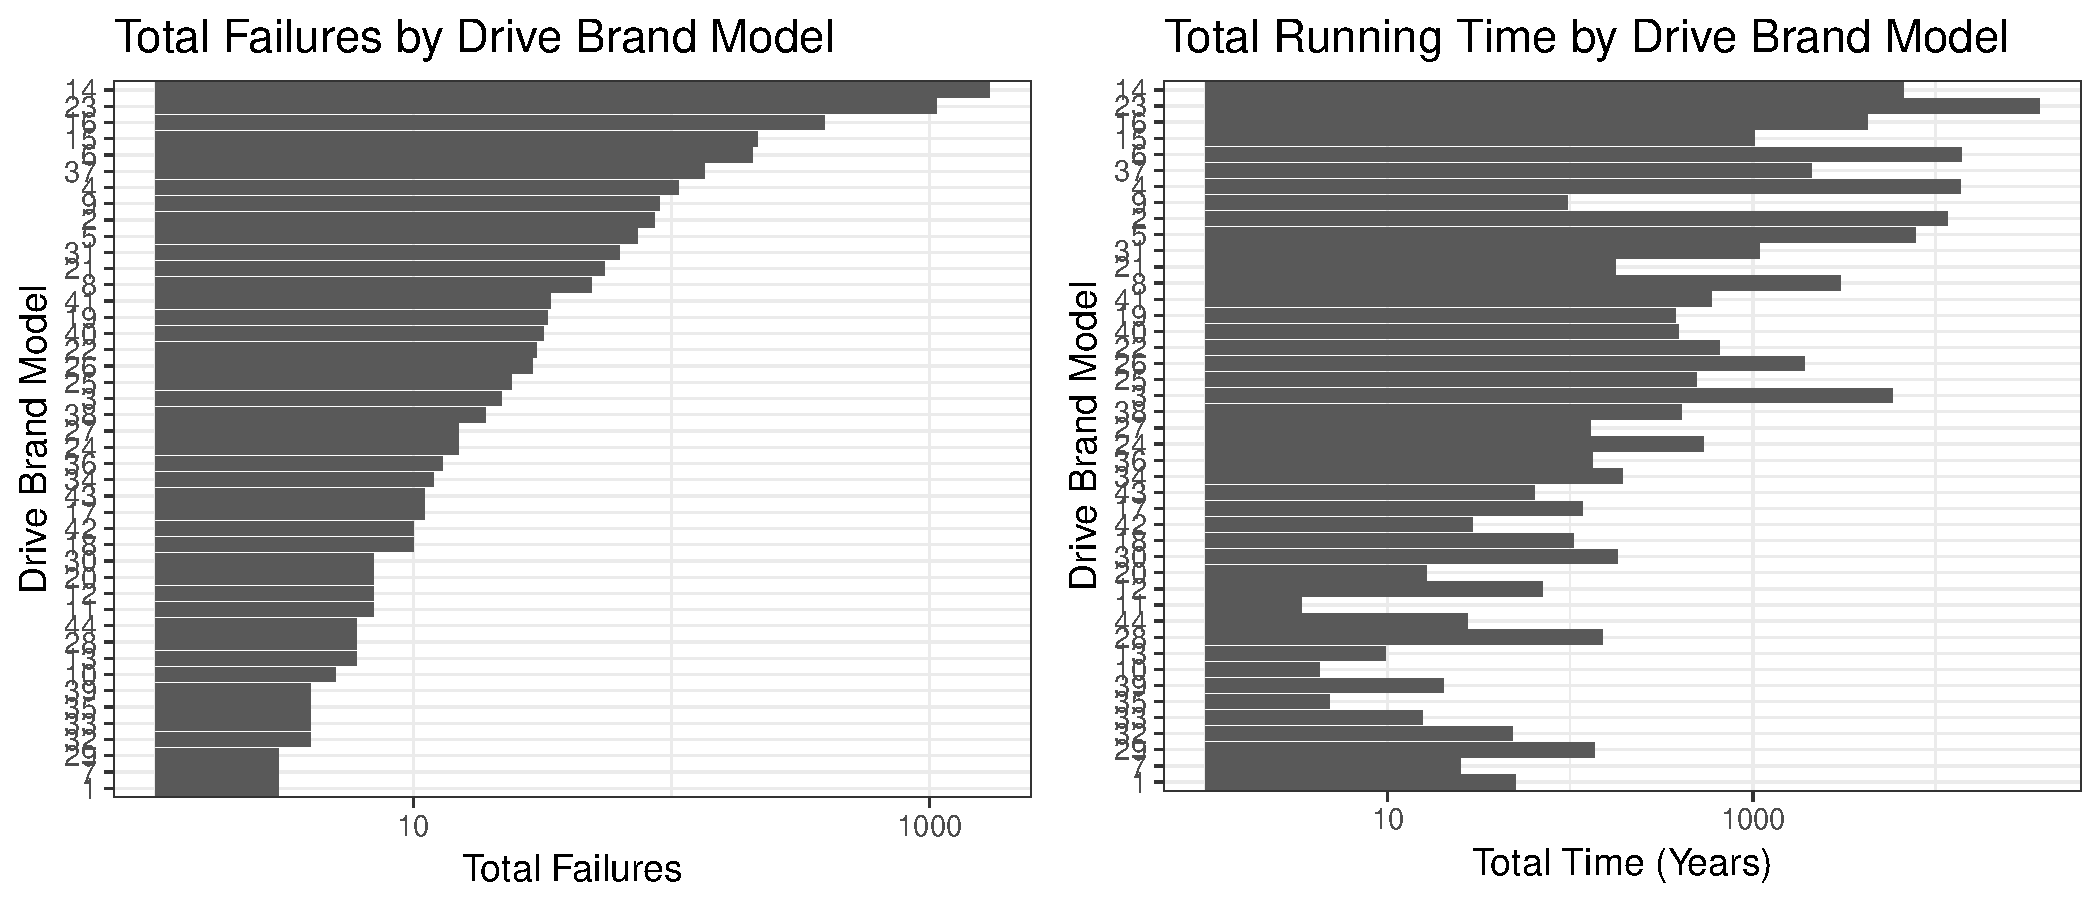
\includegraphics[width=.9\textwidth]{data-sum.pdf}
  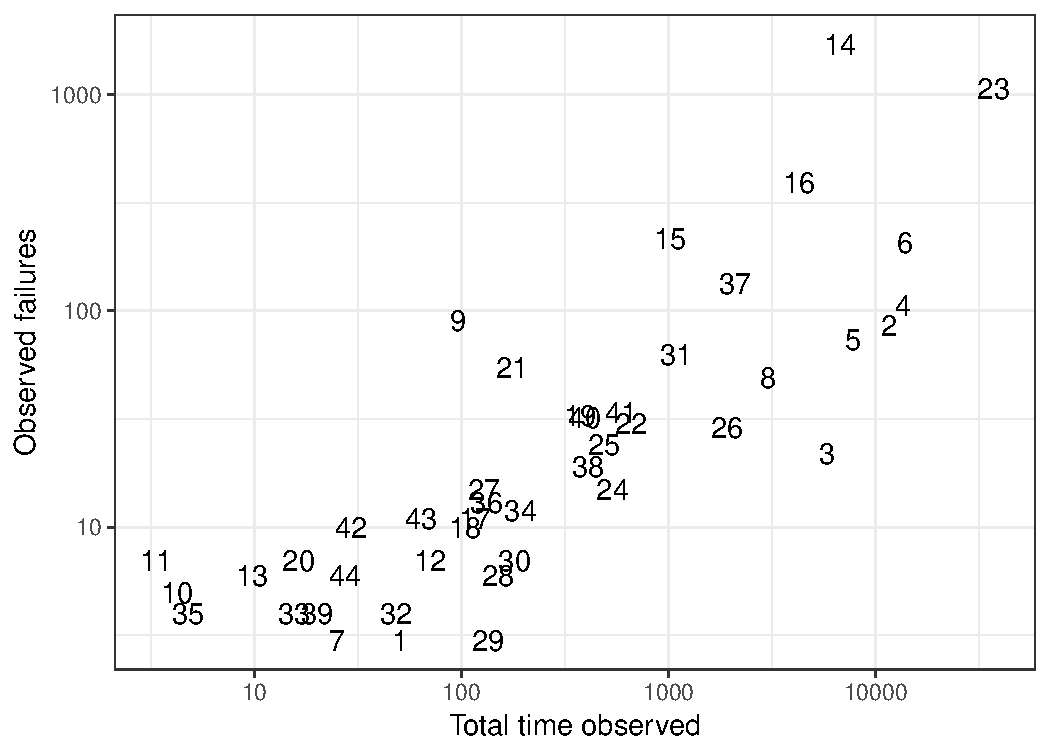
\includegraphics[width=.9\textwidth]{dm-summ-scatter.pdf}
  \caption{Scatterplot of total observed running time (hours) versus total number of observed failures.  Each number labels a unique drive brand model.}
  \label{fig1}
\end{figure}

\subsection{Modeling}
\subsubsection{Candidate Models}
We considered four models, all based on \ref{eq:hier-model}, which are identified by which model parameters are held constant across drive-models. These are (from most to least restrictive):

\begin{enumerate}
\item $\pi_{g} = \pi,\quad \mu_{1g} = \mu_1,\quad \sigma_{1g}=\sigma_1,\quad \mu_{2g} = \mu_2,\quad \sigma_{2g} = \sigma_2$
\item $\pi_{g} = \pi,\quad \mu_{1g} = \mu_1,\quad \sigma_{1g}=\sigma_1,\quad \sigma_{2g} = \sigma_2$
\item $\pi_{g} = \pi,\quad \mu_{1g} = \mu_1,\quad \sigma_{1g}=\sigma_1$
\item $\mu_{1g} = \mu_1,\quad \sigma_{1g}=\sigma_1$
\end{enumerate}

The set of model specifications were chosen based data, interpretation of the model, as well as estimation considerations.  Product specific parameters for the the wearout failure mode $(\mu_{2g},\sigma_{2g})$, and the proportion defective $(\pi_g)$, are considered as a means to account for heterogeneity across brands in the right tails of the failure distribution.  Going from a common model for all product brands and gradually increasing the complexity of the model, we end up at Model 4.  Model 4 allows for the probability of infant mortality as well as the shape and scale parameters for the 2nd failure mode to vary by product.

For all of the models we consider, the parameters for the infant mortality failure mode are held in common across products.  We found that there was often insufficient information to model these parameters hierarchically.  Moreover, assuming a common distribution for infant mortality provides a meaningful interpretation and comparison of $\pi_g$ and $\pi_{g'}$ ($g \neq g'$). 

\subsubsection{Prior Distributions}
\label{sec:Prior Distributions}
To complete the full probability model, we need to select prior distributions for the parameters governing the hierarchical model. We select proper priors to ensure a proper posterior.

For models 1-4, different sets of restrictions required different prior specifications, which were assigned as follows:

\begin{enumerate}
\item This model constrains all drive-models to the same failure distribution. For this ``reduced" model we assume the same priors as in Example 1.

\item We allow $t_{pd}$ to vary by drive-model. To help with model identifiably, we tighten the priors on the defective mode:
$$ \mbox{logit}^{-1}\pi \sim \op{Normal}(-3,1),\quad \sigma_1 \sim \op{Lognormal}(0, 1), \quad t_{p1} \sim \op{Normal}(7,2),$$
implying now a prior $90\%$ probability that $\sigma_1$ is between $0.19$ and $5.18$ and $t_{0.5,1}$ between $3.7$ and $10.3$, which, translating from the log-scale, is equivalent to an interval from 1.5 days to 3.4 years.

\item $\sigma_{d2}$ is allowed to vary. Priors for constrained parameters are the same as for model 2.

\item $\pi_d$ varies. Priors for constrained parameters are the same as for model 2.

\end{enumerate}

For the scale hyper-parameters we follow the recommendations of \citet{gelman2014bayesian} and use half-Cauchy priors. As for the location hyper-parameters, we select weakly informative priors consistent with our prior information on hard-drives. The prior for $\eta_\pi$ puts 95\% of prior mass on the interval $(0.006, 0.27)$ for the median proportion defective (What justification? Should maybe be lower.) For $\eta_{\sigma, 2}$, $95\%$ of prior mass is on values greater than $0.037$. Since $\sigma_d$ is the reciprocal of the Weibull shape parameter, this corresponds roughly to an assumption that the median Weibull shape parameter is less than $1/0.037 = 27$. The prior for $\eta_{t_{p_2},2}$ implies that the median 20th percentile for non-defective units is less than greater than 3 days and less than 24 years.

\begin{align*}
  \eta_{\pi} & \sim \op{Normal}(-3, 1)\\
  \tau_{\pi} & \sim \op{Cauchy}^+(0, 1)\\
  \eta_{\sigma ,2} & \sim \op{Normal}(0, 2)\\
  \tau_{\sigma ,2} & \sim \op{Cauchy}^+(0, 1)\\
  \eta_{t_{.2_2},2} & \sim \op{Normal}(9, 2)\\
  \tau_{t_{.2_2},2} & \sim \op{Cauchy}^+(0, 1)
 \end{align*} 

\subsection{Computation}
\label{sec:Computation}
Each model was fit using the {\tt
  rstan}\cite{rstan} package in {\tt R} \cite{r}, which implements a variant of Hamiltonian Monte Carlo (HMC)
\cite{betancourt}. HMC jointly updates all model parameters by simulating paths along the posterior density. This is done to reduce autocorrelation and efficiently explore the posterior. Multiple chains were run for 1500 iterations after 1500 warmup iterations: 4 chains were run for Models 1,2 and 3 and 16 chains were run for Model 4. The Gelman-Rubin potential scale reduction factors, ``R-hat", which test for lack of convergence by comparing the between versus within chain variability were used. Upon convergence, R-hat converges to 1. For the four model fits, the  maximum values over all the model parameters were 1.005, 1.028, 1.009 and 1.004, respectively. The minimum estimated effective sample size over all the model parameters for the four model fits were 567, 205, 672 and 3330, respectively. No divergent transitions occurred after warmup.

% HMC generates proposals by simulating paths along the posterior density. This is done to reduce autocorrelation between samples, but doing so also provides a useful diagnostic. \textit{Divergent transitions} will tend to occur when the posterior has regions of high curvature, which can present problems for MCMC by making it difficult to fully explore the posterior distribution. This feedback can be useful 



\subsection{Model Selection}
\label{sec:Model Comparisons}
The right side of Figure \ref{fig:fig2} shows that the set of estimated failure curves for all four models that we fit. The upper left panel shows the estimated failure curve fit to all data ignoring drive-model as a factor (Model 1). The upper left plot, which represents Model 2, demonstrates that there is appreciable differentiation between drive-models; note that, because the scale parameter, $\tau_{t_{p2}}$ is learned hierarchically from the data, we can ascertain that there is evidence in the data that this variability is real.

The lower left panel, representing Model 3, suggests differing shape parameters in the wearout failure mode which means that the ranking of drive-models with respect to fraction failing differs over time.

Finally, the lower right panel, corresponding to Model 4, shows that, by allowing $\pi_d$ to vary by drive-model, there is greater variability in the early rate of failure and, for some drive-models, the forecasted fraction failing is adjusted downward. 

\begin{figure}[H]
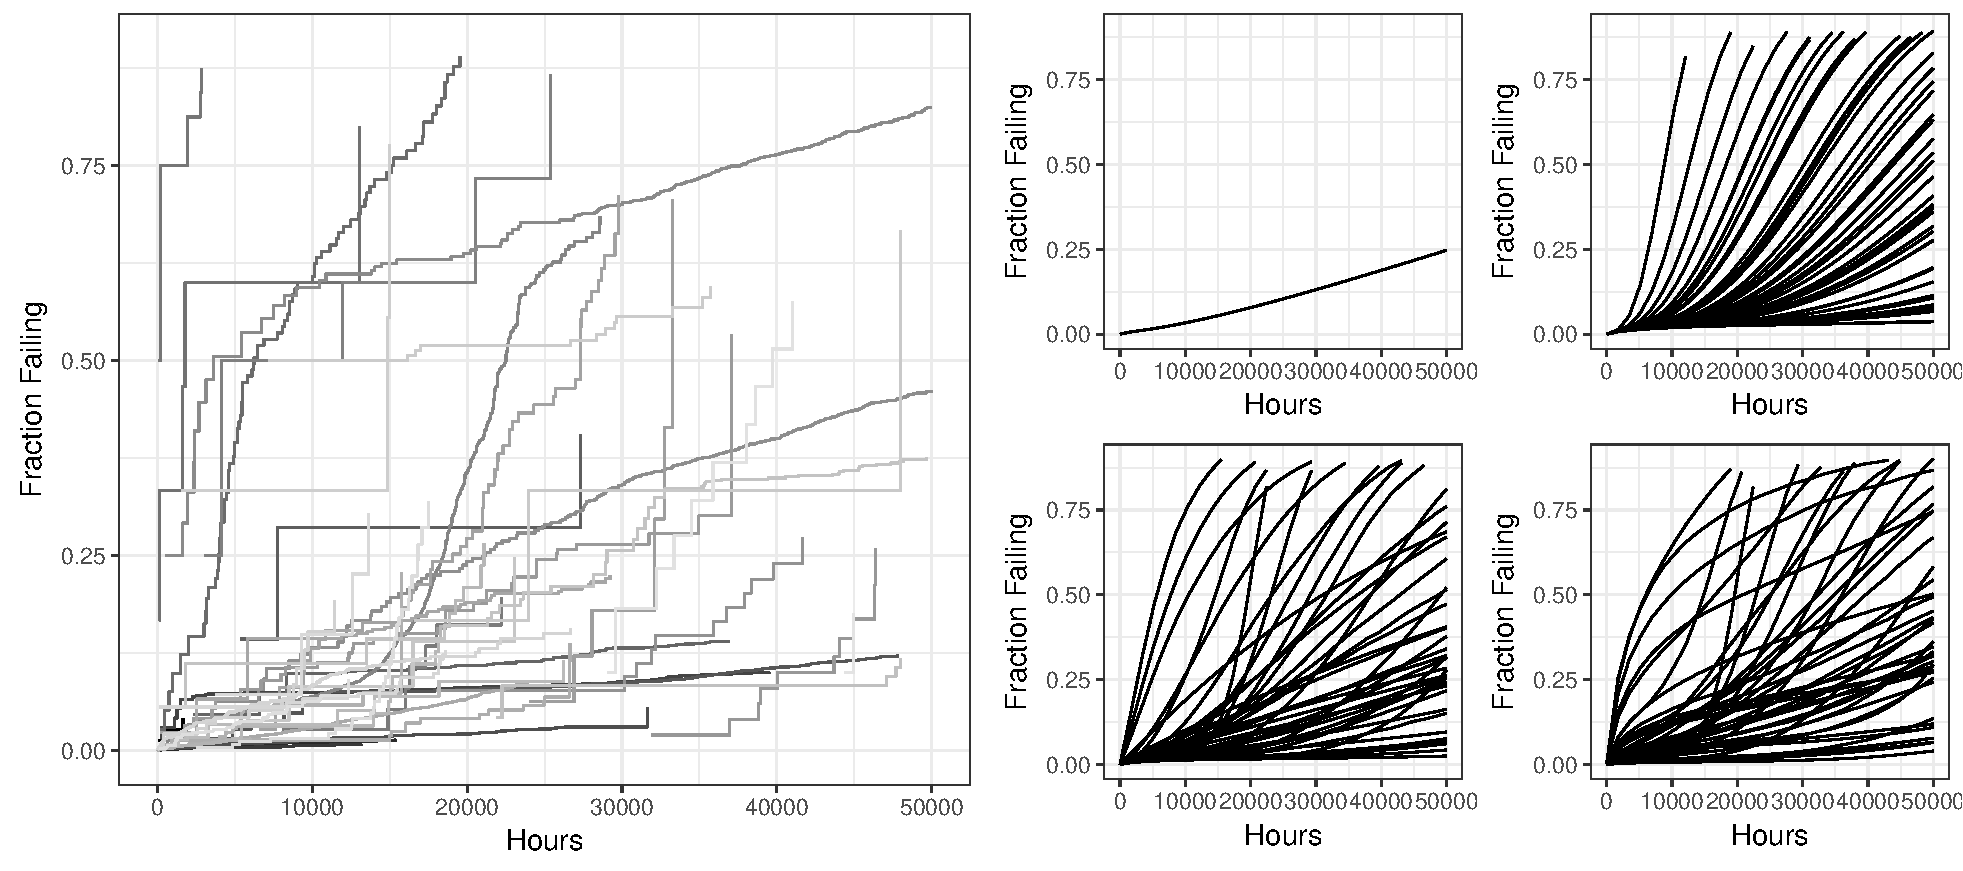
\includegraphics[width=\textwidth]{heterogeneity-compare-preliminary}
\caption{Left: Kaplan-Meier estimates of the time to failure for each of the drive-models in the Backblaze data. Right: Pointwise posterior median time to failure curves for Models 1-4, ordered left to right, top to bottom.}
\label{fig:fig2}
\end{figure}

We can also compare the model fits for each drive-model individually.  Using the set of parameters that maximize the posterior log probability, we examine the GLFP cdf for each of the 4 model specifications.  The GLFP fit for drive-models 2, 9, 14, and 40 are presented in Figure \ref{fig:mod_comp_leg}.  The black step functions again corresponds to the adjusted non-parametric estimates.  As model complexity increases, the GLFP curves become more flexible and are better able to fit the observed failure data.  All of the GLFP models appear to overestimate the proportion of failed hard drives for drive-model 2, but Model 4 agrees best with the nonparametric estimate.  For drive-model 14, Models 1-3 underestimate the proportion of drives failing, and for drive-model 40, they slightly overestimate the data.  Conversely, Model 4 follows the observed failures quite closely--accurately capturing failures at the lower and upper ends of the distribution.  The difference in accuracy between Models 3 and 4 are and Models 1 and 2 are visually quite apparent.  Differentiating between Model 3 and 4 is less clear; for instance, the fits from Model 3 and 4 line almost exactly on top of each other for drive-model 40.
\begin{figure}[H]
    \centering
   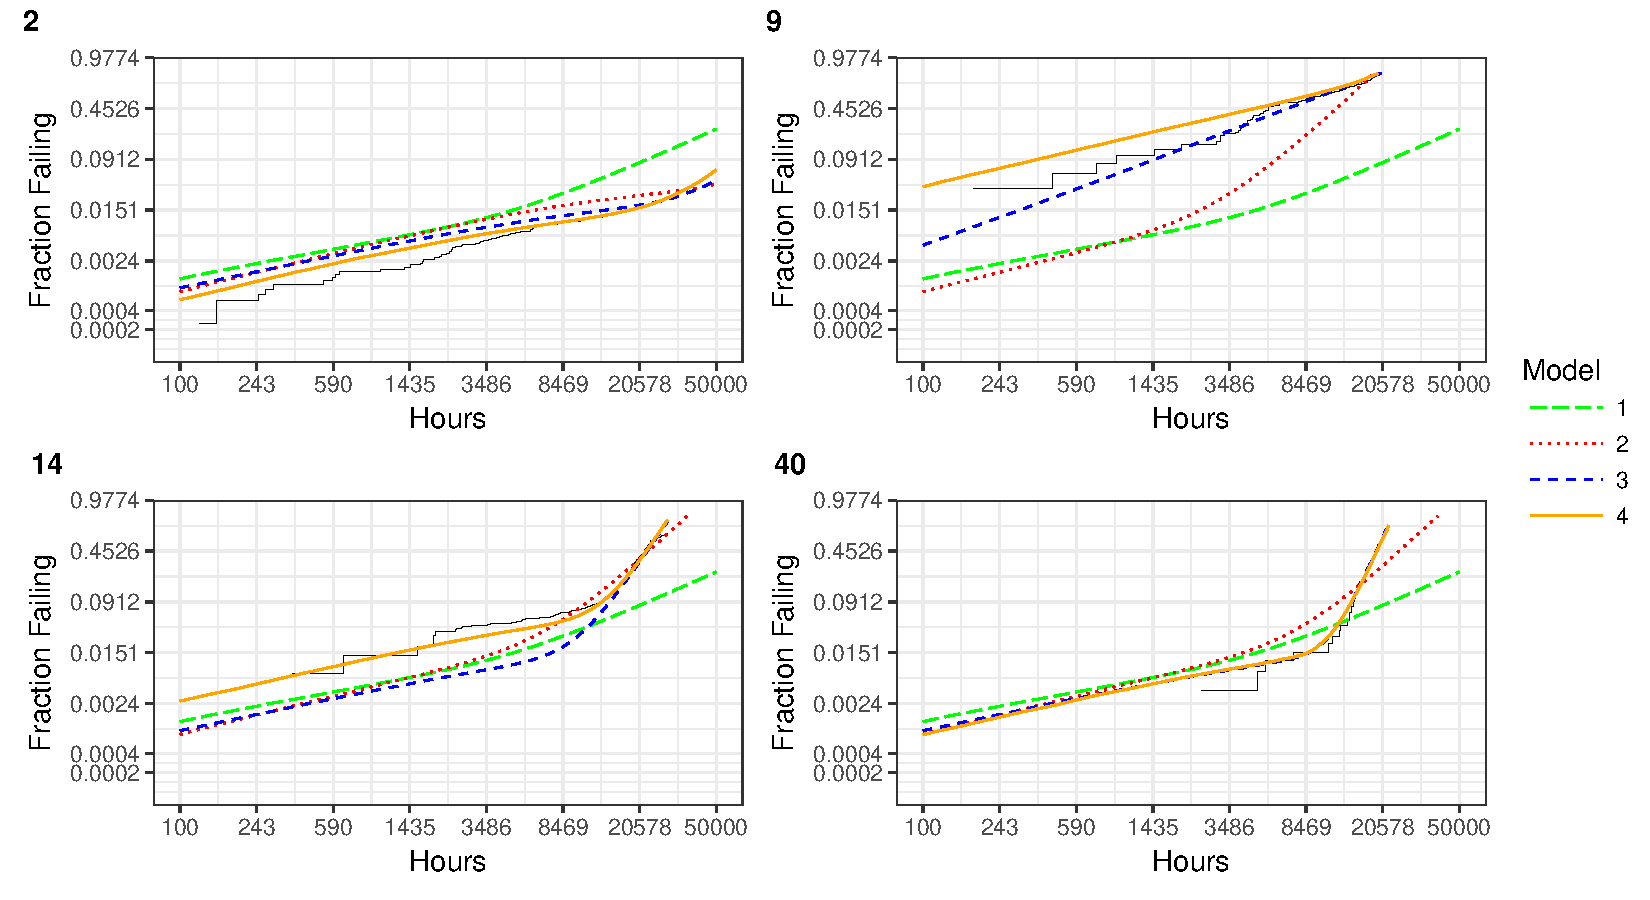
\includegraphics[width=\textwidth]{mod_compare_legend}
		\caption{Estimated GLFP for 4 drive-models plotted on Weibull paper.  The solid step function is the truncated adjusted Kaplan-Meier points.  \label{fig:mod_comp_leg}} 
\end{figure}


To statistically compare the GLFP Models, we estimated the predictive accuracy of the 4 different models using an approximate leave-one-out cross validation (LOO) method.  As outlined in Vehtari et. al, the predictive accuracy from a fitted Bayesian model can be estimated simply with posterior draws of the model parameters rather than re-fitting the model with different data sets \cite{vehtari}.  For each observation, $i$, the log point-wise predictive density is calculated over the full set of posterior samples with data point $i$ removed.  The final expected log point-wise predictive density (elpd) is the sum over all observations (elpd $=\sum{\log p(y_i|y_{-i})}$).  We computed the elpd for all 4 models using the R package loo \cite{loo}.  When $n$ is large, the distribution of the elpd is approximately normal and different models can be compared statistically.  We calculated the difference in expected predictive accuracy for Model 4 vs 3, Model 3 vs 2, and Model 2 vs 1, as well as the standard error of the difference (Table 1).  As the model complexity increased, the expected predictive accuracy improved.  Of all the models, Model 4 had the best predictive accuracy and was significantly better than the other 3 models.

\begin{table}[H]
\centering
\begin{tabular}{rrrrrrr}
  \hline
 & ELPD \ & Difference in ELPD \ & SE of the Difference \\ 
  \hline
Model 4 & -13309.5 & 40.7 & 11.3 \\ 
Model 3 & -13350.2 & 458.8 & 31.0  \\ 
Model 2 & -13809.0 & 3674.6 & 96.2 \\ 
Model 1 & -17483.6  \\ 
   \hline
\end{tabular}
\caption{Expected Log Pointwise Predictive Density (ELPD) for each model specification.  Each model is compared to the more parsimonious model below.  The estimated difference of expected leave-one-out prediction errors between the two models, as well as the standard error of the difference, is also presented.}
\label{table:1}
\end{table}

\subsection{Results}
\subsubsection{Model Assessment}
To assess the goodness of fit for our final model (Model 4), we use a graphical posterior predictive check. As stated by \citet{gelman1996postpred}, a graphical comparison of replicated data sets from the fitted model with the observed data can be very informative with regard to identification of problems with the model.

To generate replicate data sets, we must first decide what to do with regard to censoring and truncation. The representation we choose to display the data, non-parametric probability plots, guides us in making this decision. The variability of this estimator arises primarily from the number of ``at risk" units at any given time, which depends in part on these processes. Since we are not modeling the mechanisms of truncation nor censoring, we want to try to duplicate these mechanisms in the replicated data. Our method for generating a replicate data set  $y_{rep,g,i}^{(s)}$ for $s = 1 \dots 19$ is as follows:
\begin{enumerate}
\item Simulate $\tilde{y}_{rep,g,i}^{(s)} \sim \op{GLFP}(\pi_{g}^{(s)},\mu_1^{(s)},\sigma_1^{(s)},\mu_{2g}^{(s)}, \sigma_{2g}^{(s)})$.  Where each set of parameters is randomly drawn from the full posterior distribution.
\item If $\tilde{y}_{rep,g,i} < t_{g,i}^L$, then remove this time as this record is not observed
\item Define $m_{g,i}>0$ for each $g$ and $i$. If $c_{g,i}=0$, let $m_{g,i}=\max \{y_{G,i}: G=g\}$, else let $m_{g,i}=y_{g,i}$.\\
If $\tilde{y}_{rep,g,i}^{(s)}>m_{g,i}$, set $y_{rep,g,i}^{(s)}=m_{g,i},\; c_{rep,g,i}^{(s)}=1$, otherwise set $y_{rep,g,i}^{(s)}=\tilde{y}_{rep,g,i}^{(s)},\; c_{rep,g,i}^{(s)}=0$.
\end{enumerate}

We can compare the 19 simulated data sets $y_{rep,g, i}$ to the observed data $y_{g,i}$ by using them to reestimate the Kaplan-Meier nonparametric estimator. The resulting plots are displayed in figure \ref{fig:post-pred-KM}. For most drive-models, the observed estimates appear to behave similarly to those derived from the replicated data. As discussed in \ref{subsec:ex1}, drive-model 14 has a discrepancy in the right tail, which we addressed there. Drive-model 4 also appears as an exception, which we discuss now.

\begin{figure}[H]
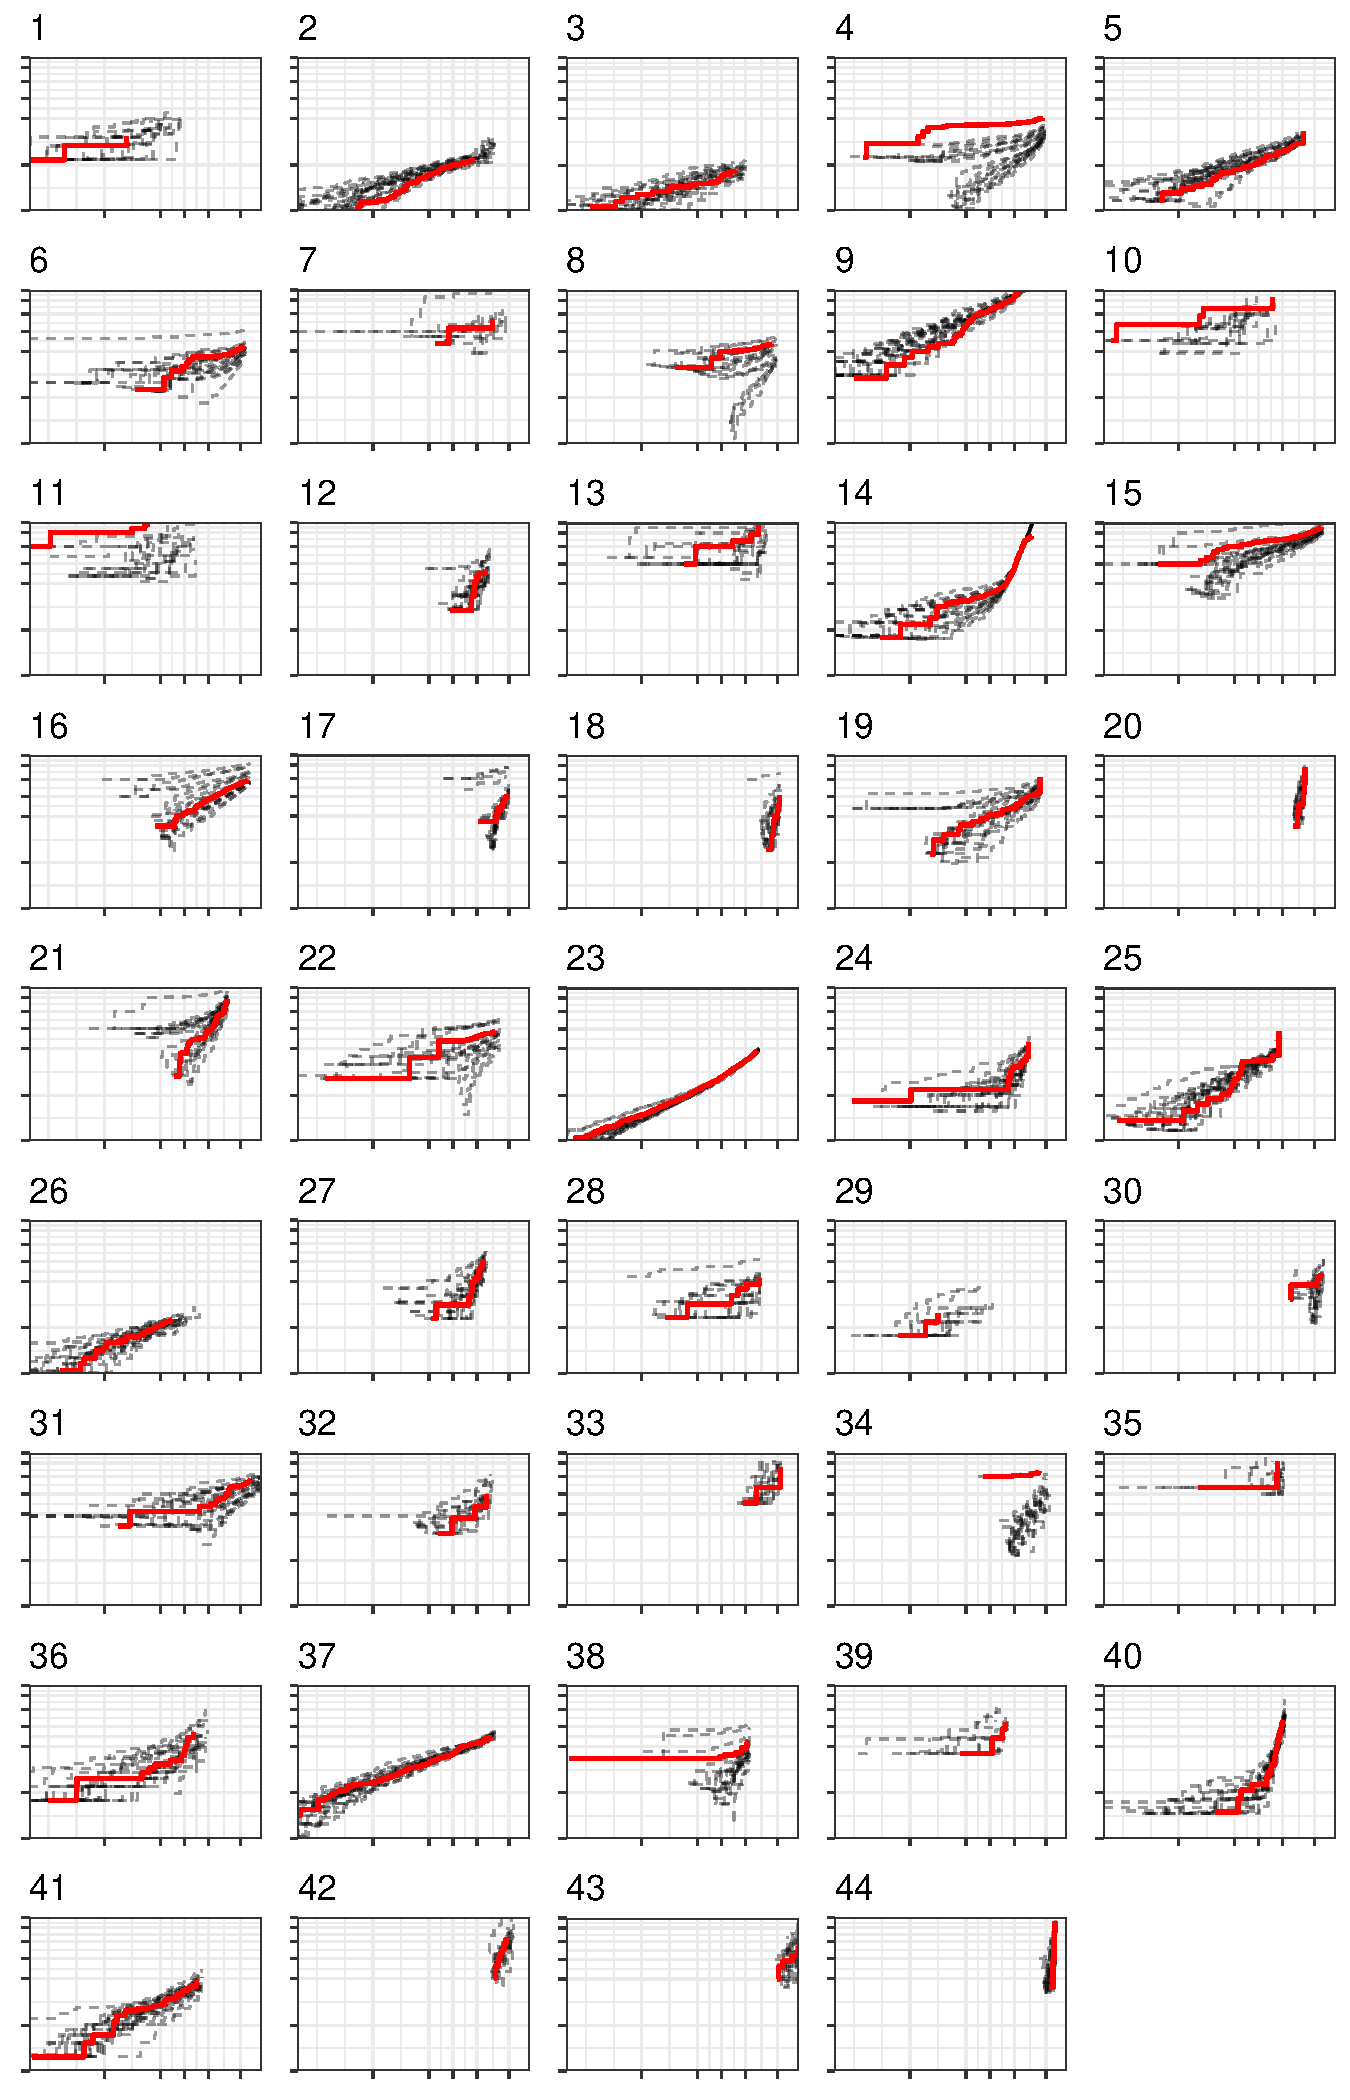
\includegraphics[width=\textwidth,height=.9\textheight]{post-pred-KM-all}
\caption{Nonparametric estimates of proportion failing for each drive-model. Both the original data (\textbf{bold} line) and 19 ``replicated" data sets from the posterior predictive distribution (\textit{dashed} lines) are shown.}
\label{fig:post-pred-KM}
\end{figure}

To better understand the reason for the discrepancy between the observed data for drive-model 4 and its posterior predictive distribution, we plot the raw data along with the truncation-adjusted nonparametric estimate of time to failure and the posterior estimate (see figure \ref{fig:ex-mod-4}). From these plots, it is clear that the large discrepancy between the posterior and the nonparametric estimate is driven by a small number of failures that occur in the first quarter year. Indeed, if we ignore records with observation periods that include the first quarter, the modified nonparametric estimate falls within the posterior 90\% pointwise credible band. Our trouble with fitting this drive-model is that while there is evidence of infant mortality in the relatively few units that were observed in the first quarter, the problem seems to go away much quicker than would be expected if there were a large number of units susceptible to the early failure mode. In any case, this example demonstrates that, conditional on the model, the weight of evidence in all the data overpowers the signal from the small sample for this drive-model, which suggests high rates infant mortality in the first quarter year.

For a clear example of this, consider drive-model 43. The data for this drive-model are heavily truncated; the observed units had run for quite some time before data were made available. In figure \ref{fig:ex-mod-43} we see that the lack of data for this drive-model at early ages results in a diffuse posterior centered around the what we call the ``global estimate," corresponding to $\op{GFLP}(\eta_{\pi}, \mu_1,\sigma_1, \eta_{t_2} - \eta_{\sigma_2}\Phi^{-1}(.2), \eta_{\sigma_2})$. Then, in the period where records exist for this drive model, at around $1\frac{1}{2}$ years, the posterior deviates from the global model, acheiving a compromise between it and the nonparametric estimate.



\begin{figure}
\centering
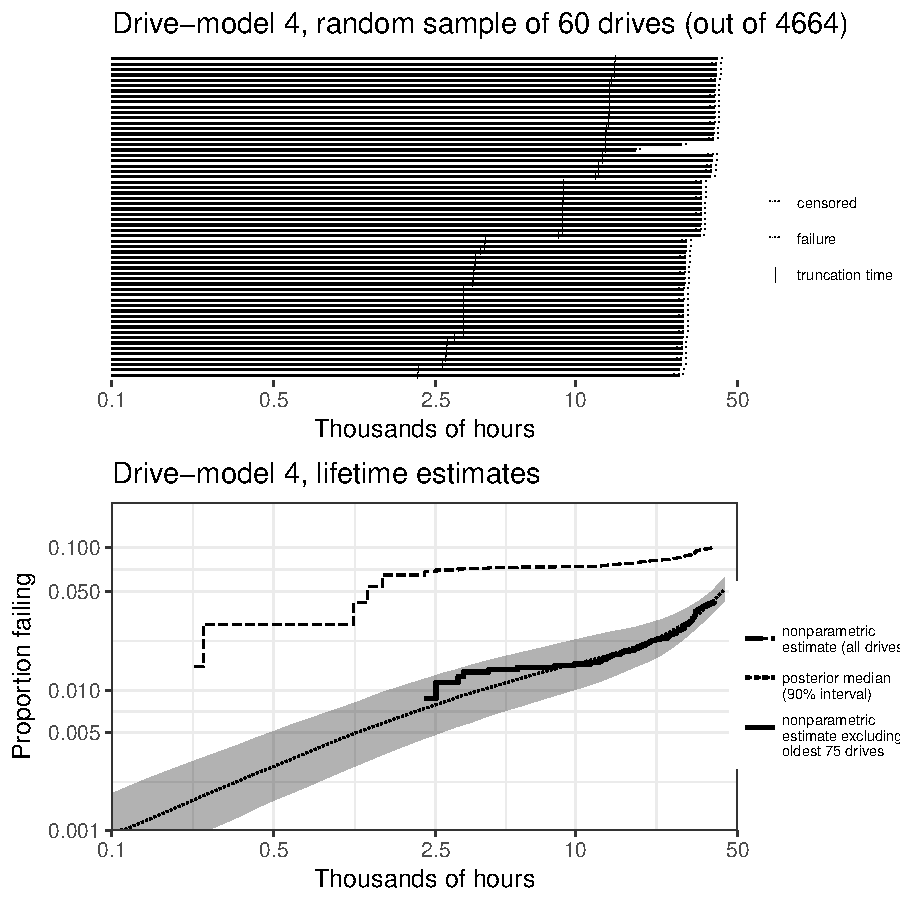
\includegraphics{dm4-exception}
\caption{Top: Graphical representation of lifetime for random sample of 200 drives of drive-model 4 from the Backblaze data set. Solid white lines indicate the observed window of life. Right-censored observations changed to a dashed line and failures mark the transition to a solid black line. Bottom: Solid step function is truncation-adjusted nonparametric estimate of the proportion failing. The dotted line is an estimate obtained after truncating the data to those starting after .25 years, with the corresponding truncation adjustment. The dashed line with gray band is pointwise posterior median, and 90\% credible interval, of proportion failing.}

\label{fig:ex-mod-4}
\end{figure}

\begin{figure}
\centering
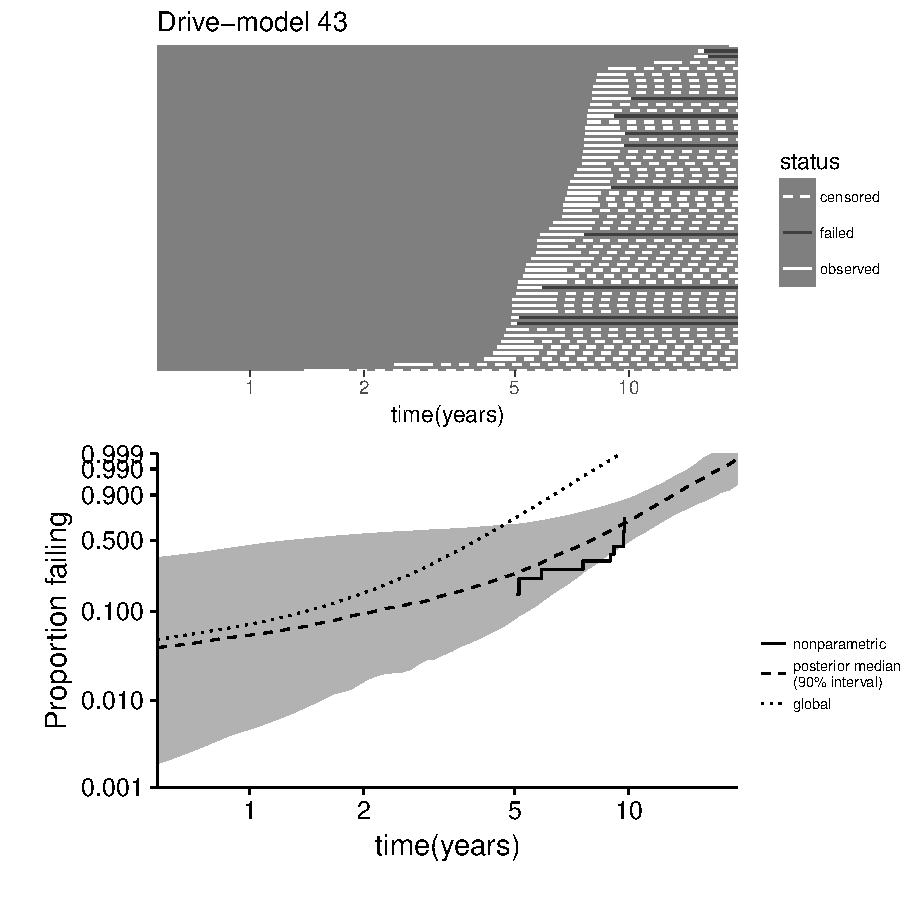
\includegraphics{dm43-shrinkage}
\caption{}
\label{fig:ex-mod-43}
\end{figure}

\subsubsection{Drive-model Comparisons}
\label{subsubsec:Drive-model Comparisons}
We consider the problem of ranking drive-models. From a
business perspective, it is clear
that we should prefer the drive-models which will provide more years
of service. For ease of exposition, we will assume that the purchase
price of a hard-drive is the same across drive-models.

There are two sources of variation at play; the
posterior uncertainty in the parameters, which largely depends on the
sample size, and the uncertainty in future
observations conditional on the parameters. The {\em posterior
  predictive} distribution incorporates both sources.
\begin{equation*}
  p(t_{d,new}|t) = \int p(t_{d,new}|\theta_d) p(\theta_d|t) \, d\theta_d
\end{equation*}

We can sample from this distribution by drawing $t_{d,new}^{(s)}$ from
$\operatorname{GLFP}(\pi_d^{(s)},
\mu_1^{(s)},\sigma_1^{(s)},\mu_{2,d}^{(s)},\sigma_{2,d}^{(s)})$, for
$s=1,...,S$, using the saved posterior draws for the model
parameters. The expected time-to-failure (TTF) for drive-model $d$ can be estimated by
$$\frac{1}{S} \sum_{s=1}^{S} t_{d,new}^{(s)}.$$

While TTF is clearly important, due to the
anticipation of advancements in technology, we can expect that the
relative value of computer hardware will depreciate rather quickly. In simple terms, given two hard drives, I would prefer to have both of them work for five years than for one to work for ten years and the other to not work at all. To account
for depreciation, rather than using TTF as the metric for drive-model comparison, we use the value at replacement. The IRS considers
computer hardware to be ``5-year'' equipment\cite{f4562}. Using``the declining
balance method'' the rate of depreciation is 40\% per year.

Let $L(t) = e^{-.4t}$ represent the value at the time of failure
relative to a new unit. We can rank the drive-models by 
$$\op{E}(L(t_{d,new})|t))\approx \frac{1}{S} \sum_{s=1}^{S} L(t_{d,new}^{(s)}).$$

Posterior credible intervals for $L(t_{d,new})$ are shown in the left panel of figure \ref{fig5}. A zoomed version of the top 8 drive-models, as ranked by $\op{E}(L(t_{d,new})|y)$ are shown in the bottom right panel. The panel above shows credible intervals for TTF. We can see that ranking by TTF would lead to a different result -- a new drive-model 8 unit expected to have the last the longest, but possibility of it failing early is higher that for the drive-models ranked highest by our depreciation-aware metric. The top four drive-models (4,5,2,3) seem very comparable, with a new drive-model 4 unit expected to depreciate the most. However, given the discrepancy of the model fit for drive-model 4, noted in the previous subsection, in the absence of more early life data, we might harbor some lingering concern about possible quality-control issues with this drive-model.

We can also use the posterior draws to compute quantiles of interest, which in reliability applications is typically more informative than a central measure of tendency.  On the left panel of Figure 5 we plot $t_{0.10}$, the .10 quantile (i.e., the amount of time it takes for 10\% of hard drives to fail), for all drive-models. The best six drive-models ranked by TTF are also the drive-models with the longest time to $t_{0.10}$.  Drive-models 5, 2, 4, and 3 seem to really stick out as the most reliable as there is a larger gap separating them from the rest of the group.  Another interesting feature to compare is $\pi$, the proportion defective.  One the right panel of Figure 5 are the posterior credible intervals of $\pi$ for each drive-model.  The plot is again sorted according to $t_{0.10}$ so it can be compared to the left hand side.  While for many of the drive-models the ordinal ranking is the same as on the left, there are some drive-model comparisons, for example 23 and 18, that differ in ranking if compared using $t_{0.10}$ or $\pi$.  Depending on a user's application or the hard drive warranty length, using the $\pi$'s as a comparison tool may be a relevant parameter of interest.   
 
\begin{figure}[H]
  \centering
  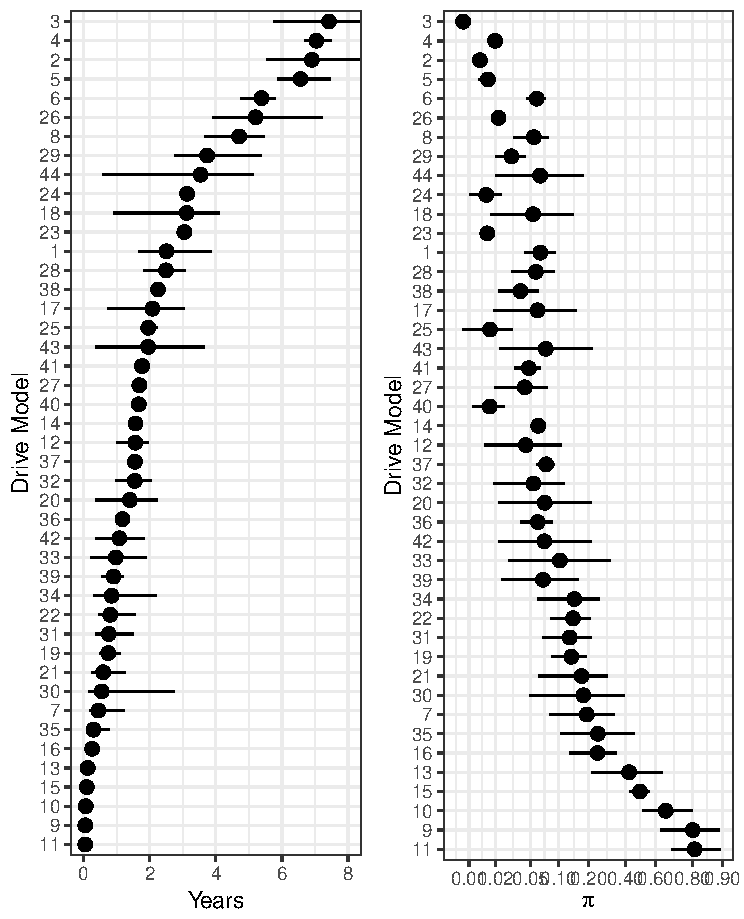
\includegraphics[width=\textwidth]{b10andpi}
  \caption{Left: 50\% credible intervals for  $t_{0.10}$ (time in years till 10\% of the drives fail). Right: 50\% credible intervals for $\pi$ plotted on the logit scale.  Both plots are sorted based on the median value of $t_{0.10}$.}
  \label{fig4}
\end{figure}

\begin{figure}[H]
  \centering
  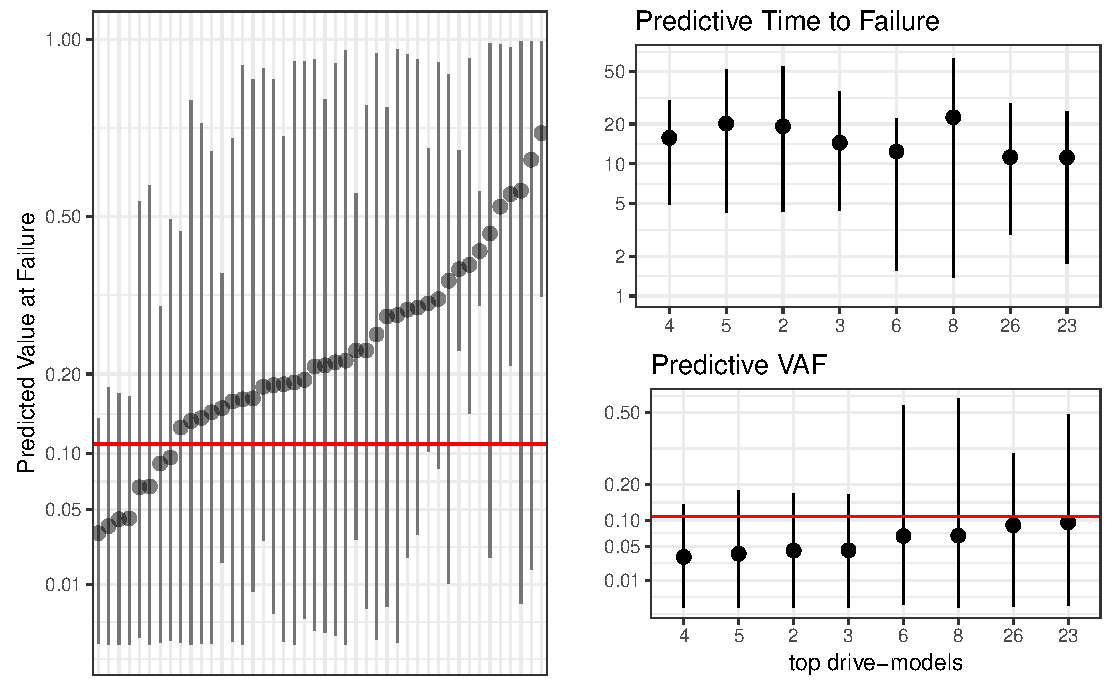
\includegraphics[width=.8\textwidth]{dm-eval}
  \caption{Left: Posterior predictive relative value-at-loss for new
    unit, by drive-model. Right: TTF (top) and VAF based on 40\% annual depreciation (bottom), for best 11 drive-models.}
  \label{fig5}
\end{figure}


\section{Conclusions}
\label{sec:Conclusions}
We should point out some assumptions made in this analysis. First, we assume exchangability of units within drive-models. This assumption is due to our ignorance about the causes of failure and of potentially important covariates. If we had information about distinguishing characteristics of the two identified failure modes, then we should use this information. Also, there could be many environmental or human-related factors that impact lifetime, such as operating conditions associated with location in the data center, which are likely confounded with drive-model.

Second, as discussed in subsection \ref{subsec:mod_assess}, if there are causes which lead to clusters of failures at spaced-out intervals, the GLFP is not flexible enough. What we assume is that the failures that occur from various causes can be approximately assigned to two phases of product life, so that the heterogeneity that we observe among drive models is due to different combinations of deficiencies. Our ignorance of the causes of failure leads us to approximate the main failure mode with a single drive-model specific Weibull distribution. Because of this, we suspect that our forecasts are too confident; especially for ``well-estimated" models, our uncertainty in the right tail of the distribution is probably too small. On the other hand, our model borrows strength across drive-models, including those with information about late failures -- information which is entirely missing in some cases. In addition, we suggest that using metrics for comparing drive-models that reduce the importance of the right tail of the distribution are appropriate for these data. With respect to decisions based on such metrics, we believe the assumptions in the previous paragraph to be the most critical. Those issues are typical to observational data such as these.

Consumers of high-tech manufactured goods usually lack the expertise to perform a failure analysis to determine the cause of failure. The ability to fit marginal models, such as GLFP, can allow investigators to answer many pertinent questions while still appropriately accounting for uncertainty and avoiding substantial model bias.

Advances in technology have made computationally intensive Bayesian methods for fitting hierarchical models feasible in practice. Hierarchical modeling can be an effective way to regularize a large number of models fits by borrowing information. Because all the data contribute some information about the global parameters, it is often sufficient to use weakly informative priors on the global parameters, making the resulting shrinkage data dependent. Using samples from the full joint posterior avoids the need for potential problematic asymptotic approximations.

Analysis using HMC is accessible to practitioners by Stan. HMC has been shown to be very efficient in effective samples per iteration because its joint updating scheme.

\section{Appendix}
\label{sec:Appendix}
We first start with a non-parametric estimate of the empirical cdf for each drive-model using the Kaplan-Meier estimator
\cite{kaplan}.  With left truncation, however, the standard Kaplan-Meier estimator for drive-model $d$, denoted by
$\widehat{F_d(t)}_{KM}$, is conditional on survival up to
$t_{d,\text{min}}^L$, the shortest reported running time of all units
of drive-model $d$ for which records are available. To produce
unconditional estimates, we adapt the adjustment method outlined by
Turnbull, and given in more detail by Meeker and Escobar
\cite{turnbull,meeker}.  For each drive-model we select
$t_{d,\text{min}}^L$, the smallest left truncated time in the sample.
By sampling from the full posterior distribution, since
$\Pr(T>t_{d,\text{min}}^L|\theta_d)$ (the probability a hard drive has
survived up to $t_{d,\text{min}}^L$) is a function of the model
parameters, we can easily compute its posterior median,
$\widehat{A}_{\text{med}} = \widehat{Pr}(T>t_{d,\text{min}}^L|\theta_d)$. We compute the adjusted estimate by

$$\widehat{F(t)}_{KMadj} = \widehat{A}_{\text{med}} + \left(1 - \widehat{A}_{\text{med}}\right)\widehat{F_d(t)}_{KM},\; t>t_{d,\text{min}}^L.$$

While this adjustment is negligible for the majority of drive-models, five drive-models receive upward adjustments of greater than 5 percent and the estimated time to failure distribution of one drive-model (30) was adjusted by nearly 16 percent, in part because the shortest truncation time for all observed units was approx. 2.3 years.

\pagebreak

\begin{center}
{\large\bf SUPPLEMENTARY MATERIAL}
\end{center}

\begin{description}

\item Put R Stan code here

\end{description}

\begin{appendix}
\scriptsize
\begin{verbatim}
functions {
  real sev_logpdf(real y, real mu, real sigma){
    real z;
    z = (y - mu) / sigma;
    return -log(sigma) + z - exp(z);
  }
  
  real sev_logccdf(real y, real mu, real sigma){
    return -exp((y - mu) / sigma);
  }
  
  real sev_logcdf(real y, real mu, real sigma){
    return log1m_exp(-exp((y - mu) / sigma));
  }
}

data {
  int M;
  int N_obs;
  int N_cens;
  real endtime_obs[N_obs];
  real endtime_cens[N_cens];
  real starttime_obs[N_obs];
  real starttime_cens[N_cens];
  int<lower=1, upper=M> dm_obs[N_obs];
  int<lower=1, upper=M> dm_cens[N_cens];
  vector<lower=0, upper=1>[2] p; # quantiles to model
}
transformed data{
  vector[2] z_corr;
  for(i in 1:2)
    z_corr[i] = log(-1.0 * log1m(p[i])); # used to get location(mu) from quantile(t_p)
}
parameters{
  real log_tp1;
  real<lower=0> sigma1;
  real eta_tp2;
  real eta_s2;
  real eta_pi;
  real<lower=0> tau_tp2;
  real<lower=0> tau_s2;
  real<lower=0> tau_pi;
  vector[M] log_tp2_raw;
  real<lower=0, upper=1> sigma2[M];
  vector[M] logit_pi_raw;
}

transformed parameters{
  real mu1;
  vector[M] mu2;
  vector[M] log_pi;
  mu1 = log_tp1 - sigma1 * z_corr[1];
  for(m in 1:M){
    mu2[m] = (eta_tp2 + tau_tp2 * log_tp2_raw[m]) - (sigma2[m] * z_corr[2]);
  }
  for(m in 1:M)
    log_pi[m] = log_inv_logit(eta_pi + tau_pi * logit_pi_raw[m]);
}

model{
  real tmp[2];
  int m;
  real logpi;
  real mu_1;
  real mu_2;
  real sig_1;
  real sig_2;
  
  for(i in 1:N_obs){
    m = dm_obs[i];
    logpi = log_pi[m];
    mu_2 = mu2[m];
    sig_2 = sigma2[m];
    // numerator:   log( p * f1 * (1 - F2) + f2 * (1 - p * F1) )
    //            = log( exp(log(p) + log(f1) + log(1 - F2)) + exp(log(f2) + log(1 - exp(log(p) + log(F1)))) )
    tmp[1] = log_sum_exp(logpi + sev_logpdf(endtime_obs[i], mu1, sigma1) +
               sev_logccdf(endtime_obs[i], mu_2, sig_2),
               sev_logpdf( endtime_obs[i], mu_2, sig_2) + 
               log1m_exp(logpi + sev_logcdf(endtime_obs[i], mu1, sigma1)
               )
             );
    // denominator:  log((1 - p * F1) * (1 - F2))
    //            =  log(1 - p * F1) + log(1 - F2)
    tmp[2] = log1m_exp(logpi + sev_logcdf(starttime_obs[i], mu1, sigma1)) + 
             sev_logccdf(starttime_obs[i], mu_2, sig_2);
             
    target += tmp[1] - tmp[2];
  }
  
  for(i in 1:N_cens){
    m = dm_cens[i];
    logpi = log_pi[m];
    mu_2 = mu2[m];
    sig_2 = sigma2[m];
  
    // numerator:   log((1 - p * F1) * (1 - F2))
    //            =  log(1 - p * F1) + log(1 - F2)
    tmp[1] = log1m_exp(logpi + sev_logcdf(endtime_cens[i], mu1, sigma1)) + 
             sev_logccdf(endtime_cens[i], mu_2, sig_2);
    // denominator:  log((1 - p * F1) * (1 - F2))
    //            =  log(1 - p * F1) + log(1 - F2)
    tmp[2] = log1m_exp(logpi + sev_logcdf(starttime_cens[i], mu1, sigma1)) + 
             sev_logccdf(starttime_cens[i], mu_2, sig_2);
             
    target += tmp[1] - tmp[2];
  }
  
  log_tp1        ~ normal(7, 2);
  log_tp2_raw    ~ normal(0, 1);
  sigma1         ~ lognormal(0, 1);
  sigma2         ~ lognormal(eta_s2, tau_s2);
  logit_pi_raw   ~ normal(0, 1);
  eta_tp2       ~ normal(9, 2);
  eta_s2         ~ normal(0, 2);
  eta_pi         ~ normal(-3, 1);
  tau_tp2       ~ cauchy(0,1);
  tau_s2         ~ cauchy(0,1);
  tau_pi         ~ cauchy(0,1);
}

\end{verbatim}
\end{appendix}

\pagebreak

\bibliographystyle{apalike}
\bibliography{sample}

\end{document}
